% !TEX TS-program = pdflatex
% Source of Graphics/PlotGood.pdf, the well-drawn plot in Chapter 4 of the
% sample. It is made with pgfplots; compile it on its own with pdflatex.
% It is drawn at its printed size, 4 in wide, so it is included without a
% width option; its labels are in the Times font of the text, at 10 pt.
\documentclass[10pt,border=2pt]{standalone}
\usepackage[T1]{fontenc}
\usepackage{newtxtext,newtxmath}
\usepackage{pgfplots}
\pgfplotsset{compat=1.16}
\begin{document}
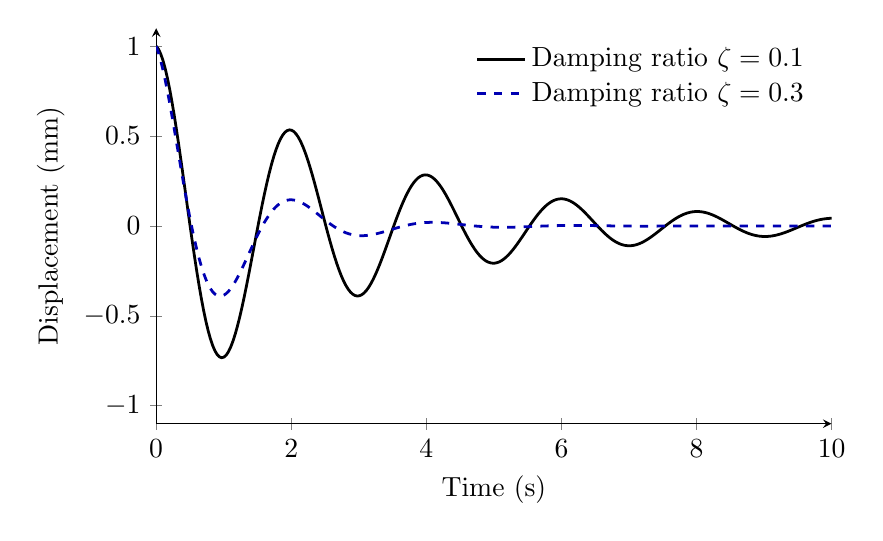
\begin{tikzpicture}
\begin{axis}[
  width=4in, height=2.6in,
  xlabel={Time (s)}, ylabel={Displacement (mm)},
  xmin=0, xmax=10, ymin=-1.1, ymax=1.1,
  ytick={-1,-0.5,0,0.5,1},
  y tick label style={/pgf/number format/.cd, fixed, precision=1},
  axis lines=left,
  legend cell align=left,
  legend style={draw=none, fill=white, fill opacity=0.8, text opacity=1,
                at={(0.98,0.98)}, anchor=north east},
]
\addplot[black, line width=1pt, samples=300, domain=0:10]
  {exp(-0.1*2*pi*0.5*x)*cos(deg(2*pi*0.5*sqrt(1-0.01)*x))};
\addplot[blue!70!black, line width=1pt, dashed, samples=300, domain=0:10]
  {exp(-0.3*2*pi*0.5*x)*cos(deg(2*pi*0.5*sqrt(1-0.09)*x))};
\legend{Damping ratio $\zeta = 0.1$, Damping ratio $\zeta = 0.3$}
\end{axis}
\end{tikzpicture}
\end{document}
